
\section{Exemples}


\begin{frame}
 \frametitle{DGtal v0.2}

 \small
 \begin{exampleblock}{}
   \centering  Noyau de base
 \end{exampleblock}
 \begin{columns}
   \column{5.5cm}
   
   
   \begin{block}{Types et structures de donn�es de base\HH}
     Espace discret, points, vecteurs (nD)
     
     trace, concepts
   \end{block}
   
   
   \column{5.5cm}
   
   \begin{block}{Repr�sentation des images\HH}
     Image container by : STL Vectors, STL Map, Hashtree 
   \end{block}
    \end{columns}
 
 \begin{center}
   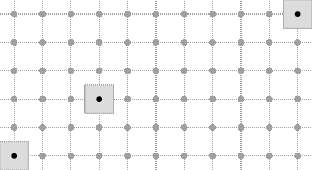
\includegraphics[width=3.5cm]{dgtalboard-1-points.png}~~~~~~~~~~~~~~~~ 
   \includegraphics[width=3cm]{hashtree}
 \end{center}
\end{frame}


\begin{frame}
  \frametitle{DGtal v0.2}
  
 \begin{exampleblock}{}
   \centering  Modules de base       
 \end{exampleblock}
 \begin{columns}
   \column{5cm}
   \begin{block}{Module topologique\HH}       
     \begin{itemize}
     \item Topologie digitale : ensembles, connexit�, bords,
       compos. connexes
     \item Points simples
     \end{itemize}
   \end{block}
   
   
   \column{5cm}
   \begin{block}{Module g�om�trique\HH}       
     \begin{itemize}
      
     \item Primitives g�om�triques : DSS (8,4, O'Rourke)
     \item Analyse contour : GreedyDecomposition
     \item Analyse volumique : DT (n-D optimale)
     \end{itemize}
   \end{block}
   
 \end{columns}
 

 \begin{center}
   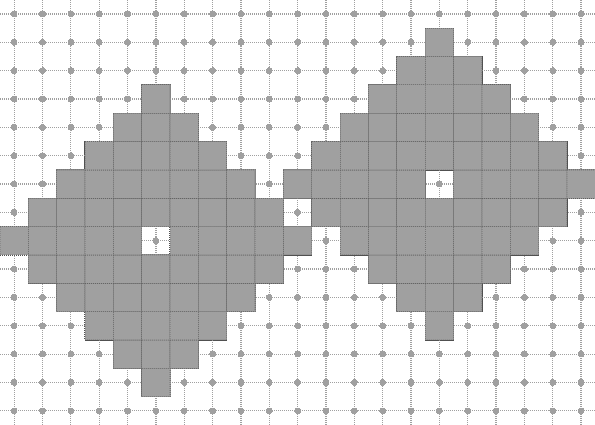
\includegraphics[width=2.5cm]{dgtalboard-2-sets-1.png}~~~~ 
   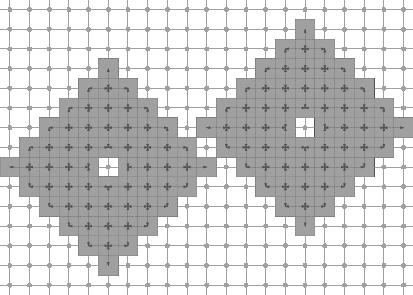
\includegraphics[width=2.5cm]{dgtalboard-2-sets-2.png}~~~~
   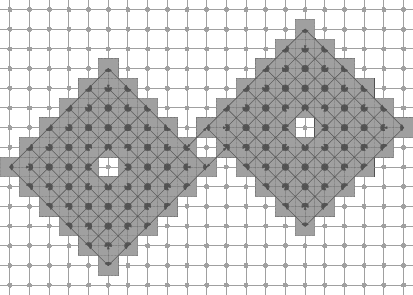
\includegraphics[width=2.5cm]{dgtalboard-2-sets-3.png}~~~~
   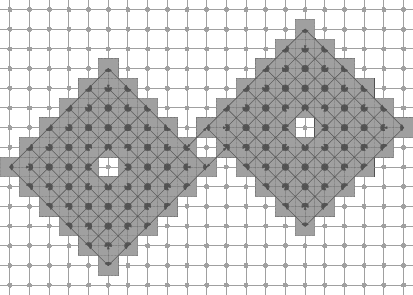
\includegraphics[width=2.5cm]{dgtalboard-2-sets-3.png}\\
   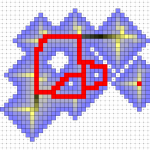
\includegraphics[width=1.7cm]{shape-thinning-4-8-150x150.png}~~~~
   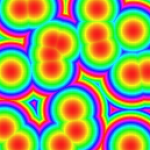
\includegraphics[width=1.7cm]{image-postDT-border-150x150.png}~~~~
   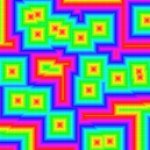
\includegraphics[width=1.7cm]{image-DT-linfty-150x150.png}~~~~
   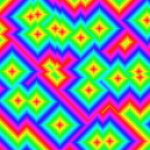
\includegraphics[width=1.7cm]{image-DT-l1-150x150.png}~~~~
   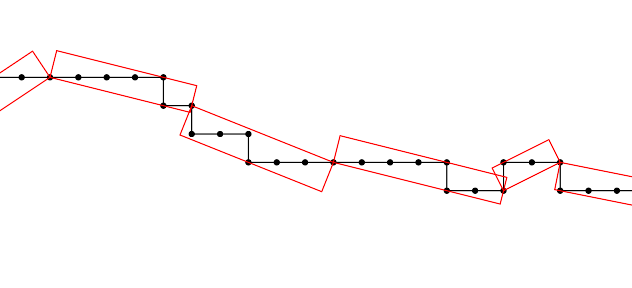
\includegraphics[width=3cm]{segmentation}~~~~
 \end{center}
\end{frame}

\begin{frame}
  \frametitle{DGtal v0.2}
 
 \begin{exampleblock}{}  
   \centering Autres modules      
 \end{exampleblock}
 
 \begin{block}{Entr�es/sorties\HH} 
   \begin{itemize}
   \item 2D: pnm, raw, + beaucoup formats (si ImageMagick install�)
   \item 3D: raw, Vol
   \item nD: raw + serialisation avec boost        
   \end{itemize}
 \end{block}
 
\end{frame}

\begin{frame}


exemples...

\begin{itemize}
\item digitalset + board (dgtal-2-sets-*.cpp)
\item DSS reco/decomp
\item distancetransform2D
\end{itemize}
\end{frame}



